\documentclass[a4paper]{article}

\usepackage{amsmath}
\usepackage{amssymb}
\usepackage{cancel}
\usepackage{stellar}
\usepackage{parskip}
\usepackage{fullpage}
\usepackage{tikz}
\usepackage{wrapfig}
\usepackage{xfrac}
\usepackage{witharrows}
\usepackage{mathrsfs}

\WithArrowsOptions{displaystyle}

\usetikzlibrary{calc}
\usetikzlibrary{decorations.markings}
\usetikzlibrary{cd}
\usetikzlibrary{positioning}
\usetikzlibrary{decorations.pathmorphing}


% Cancel color
\renewcommand{\CancelColor}{\color{red}}

\title{Graphs}
\author{Paolo Bettelini}
\date{}

\begin{document}

\maketitle
\tableofcontents

\section{Introduzione ai grafi}

\subsection{Il problema dei ponti di Königsberg}

\begin{radioactive}
    Il problema dei ponti di Königsberg consiste nello stabilire se sia possibile fare una passeggiata che attraversi ogni ponte una e una sola volta, eventualmente ritornando al punto di partenza.
    L'idea fondamentale è che non conta la forma precisa delle regioni o dei ponti: conta solo quali regioni sono collegate da quali ponti. Rappresentiamo quindi le regioni con punti, detti \emph{vertici}, e i ponti con archi, detti \emph{lati}.
    Questo grafo non è semplice: tra due regioni possono esserci più ponti, quindi nel grafo compaiono lati multipli.
\end{radioactive}

\begin{radioactive}
\begin{center}
    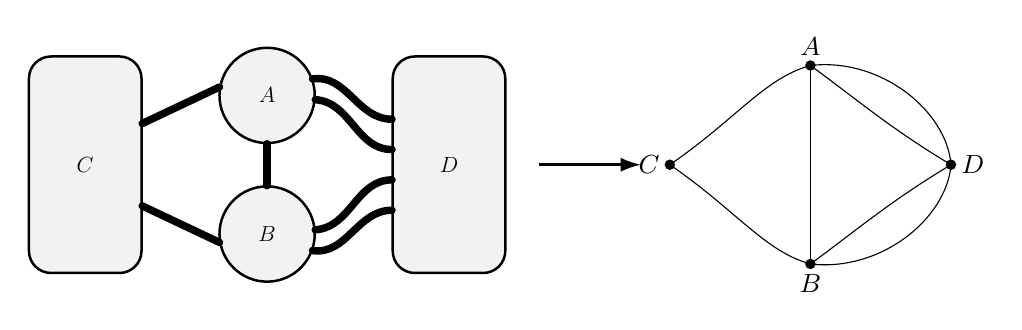
\begin{tikzpicture}[
        >=Latex,
        every node/.style={font=\small},
        land/.style={draw=black, line width=0.9pt, fill=gray!10},
        bridge/.style={
            draw=black,
            double=black,
            double distance=2pt,
            line width=0.35pt,
            line cap=round
        }
    ]

    \begin{scope}[scale=0.55, transform shape]
        \node[land, rounded corners=8pt,
            minimum width=2.6cm, minimum height=5.0cm] (LC) at (-4.2,0) {};

        \node[land, circle, minimum size=2.2cm] (LA) at (0,1.6) {};

        \node[land, circle, minimum size=2.2cm] (LB) at (0,-1.6) {};

        \node[land, rounded corners=8pt,
            minimum width=2.6cm, minimum height=5.0cm] (LD) at (4.2,0) {};

        \coordinate (LCA)  at ($(LC.east)+(0,0.95)$);
        \coordinate (LCB)  at ($(LC.east)+(0,-0.95)$);

        \coordinate (LDAu) at ($(LD.west)+(0,1.05)$);
        \coordinate (LDAl) at ($(LD.west)+(0,0.35)$);
        \coordinate (LDBu) at ($(LD.west)+(0,-0.35)$);
        \coordinate (LDBl) at ($(LD.west)+(0,-1.05)$);

        \draw[bridge] (LCA) -- (LA.170);
        \draw[bridge] (LCB) -- (LB.190);
        \draw[bridge] (LA.-90) -- (LB.90);

        \draw[bridge] (LA.20)  to[out=8,in=180]  (LDAu);
        \draw[bridge] (LA.-5)  to[out=-4,in=180] (LDAl);

        \draw[bridge] (LB.5)   to[out=4,in=180]  (LDBu);
        \draw[bridge] (LB.-20) to[out=-8,in=180] (LDBl);

        \node at (LC) {\Large \(C\)};
        \node at (LA) {\Large \(A\)};
        \node at (LB) {\Large \(B\)};
        \node at (LD) {\Large \(D\)};
    \end{scope}

    \draw[line width=0.9pt, -{Latex[length=2.6mm,width=1.8mm]}]
        (3.45,0) -- (4.75,0);

    \begin{scope}[xshift=6.9cm, scale=1.05, transform shape]
        \coordinate (RA) at (0,1.2);
        \coordinate (RB) at (0,-1.2);
        \coordinate (RC) at (-1.7,0);
        \coordinate (RD) at (1.7,0);

        \fill (RA) circle (1.8pt);
        \fill (RB) circle (1.8pt);
        \fill (RC) circle (1.8pt);
        \fill (RD) circle (1.8pt);

        \node[above] at (RA) {\(A\)};
        \node[below] at (RB) {\(B\)};
        \node[left]  at (RC) {\(C\)};
        \node[right] at (RD) {\(D\)};

        \draw (RC) .. controls (-0.9,0.55) and (-0.55,1.05) .. (RA);
        \draw (RC) .. controls (-0.9,-0.55) and (-0.55,-1.05) .. (RB);

        \draw (RA) .. controls (0.55,0.8) and (0.95,0.45) .. (RD);
        \draw (RA) .. controls (0.85,1.3) and (1.65,0.65) .. (RD);

        \draw (RB) .. controls (0.55,-0.8) and (0.95,-0.45) .. (RD);
        \draw (RB) .. controls (0.85,-1.3) and (1.65,-0.65) .. (RD);

        \draw (RA) -- (RB);
    \end{scope}

    \end{tikzpicture}
\end{center}
\end{radioactive}

\begin{snippetdefinition}{Grafo}
    Un \emph{grafo} \(G\) è formato dai seguenti dati:
    \begin{itemize}
        \item un insieme \(V\), i cui elementi sono detti \emph{vertici};
        \item un insieme \(E\), i cui elementi sono detti \emph{lati};
        \item una funzione che associa a ogni lato \(e\in E\) una coppia non ordinata di vertici, detti \emph{estremi} del lato.
    \end{itemize}

    Non si esclude la possibilità che i due estremi coincidano. In tal caso il lato si chiama \emph{cappio}.
\end{snippetdefinition}

\[
    \begin{tikzpicture}[scale=1]
        \coordinate (v) at (0,0);
        \fill (v) circle (1.8pt);
        \draw (v) .. controls +(0.6,0.6) and +(-0.6,0.6) .. (v);
        \node[below] at (v) {\(v\)};
    \end{tikzpicture}
\]

\begin{snippetdefinition}{Grafo semplice}
    Un grafo si dice \emph{semplice} se:
    \begin{itemize}
        \item non ha cappi;
        \item non ha lati multipli, cioè non esistono due lati distinti con gli stessi estremi.
    \end{itemize}
\end{snippetdefinition}

Alcuni autori chiamano \emph{grafo} ciò che qui chiamiamo grafo semplice, e chiamano \emph{multigrafo} un grafo in cui sono ammessi cappi e lati multipli.

\begin{snippetdefinition}{Grafo finito}
    Un grafo \(G=(V,E)\) si dice \emph{finito} se sia \(V\) sia \(E\) sono insiemi finiti.
\end{snippetdefinition}

\begin{snippetdefinition}{Adiacenza e valenza}
    Due vertici \(u,v\in V\) si dicono \emph{adiacenti} se sono estremi di uno stesso lato.

    La \emph{valenza}, o \emph{grado}, di un vertice \(v\), indicata con
    \[
        \deg(v),
    \]
    è il numero di lati che hanno \(v\) come estremo. I cappi si contano due volte, perché un cappio ha entrambi gli estremi uguali a \(v\).
\end{snippetdefinition}

\begin{snippetexample}{Calcolo delle valenze}
    Consideriamo il seguente grafo.

    \[
        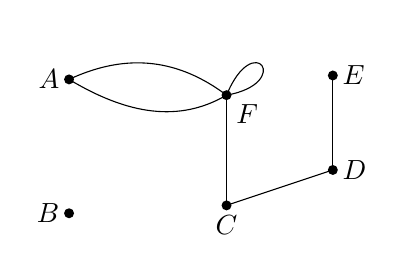
\begin{tikzpicture}[scale=1]
            \coordinate (A) at (-2,0.8);
            \coordinate (B) at (-2,-0.9);
            \coordinate (F) at (0,0.6);
            \coordinate (C) at (0,-0.8);
            \coordinate (D) at (1.35,-0.35);
            \coordinate (E) at (1.35,0.85);

            \node[left] at (A) {\(A\)};
            \node[left] at (B) {\(B\)};
            \node[below right] at (F) {\(F\)};
            \node[below] at (C) {\(C\)};
            \node[right] at (D) {\(D\)};
            \node[right] at (E) {\(E\)};

            \draw (A) .. controls (-1.25,1.15) and (-0.6,1.05) .. (F);
            \draw (A) .. controls (-1.25,0.35) and (-0.6,0.25) .. (F);
            \draw (F)--(C);
            \draw (C)--(D);
            \draw (D)--(E);
            \draw (F) .. controls +(0.35,0.85) and +(0.85,0.15) .. (F);

            \foreach \p in {A,B,C,D,E,F}{
                \fill (\p) circle (1.8pt);
            }
        \end{tikzpicture}
    \]

    Le valenze dei vertici sono:
    \[
        \begin{array}{c|cccccc}
            v & A & B & C & D & E & F \\
            \hline
            \deg(v) & 2 & 0 & 2 & 2 & 1 & 5
        \end{array}
    \]
    Il vertice \(B\) è isolato, quindi ha valenza \(0\). Il vertice \(F\) ha valenza \(5\), perché i due lati paralleli verso \(A\) contribuiscono \(2\), il lato verso \(C\) contribuisce \(1\), e il cappio contribuisce \(2\).
\end{snippetexample}

\begin{snippetproposition}{Lemma della stretta di mano}
    Sia \(G=(V,E)\) un grafo finito. Allora
    \[
        \sum_{v\in V}\deg(v)=2\cardinality{E}.
    \]
    In particolare, il numero di vertici di valenza dispari è pari.
\end{snippetproposition}

\begin{snippetproof}{}
    Elencando tutti i lati e, per ciascuno di essi, i suoi estremi, ogni lato contribuisce esattamente \(2\) alla somma delle valenze. Infatti un lato ordinario contribuisce \(1\) a ciascuno dei suoi due estremi, mentre un cappio contribuisce \(2\) al suo unico estremo.

    Quindi
    \[
        \sum_{v\in V}\deg(v)=2\cardinality{E}.
    \]
    Il membro di destra è pari. D'altra parte, nella somma delle valenze, i vertici di valenza pari contribuiscono con addendi pari, mentre i vertici di valenza dispari contribuiscono con addendi dispari. Una somma di interi è pari se e solo se contiene un numero pari di addendi dispari. Dunque il numero di vertici di valenza dispari è pari.
\end{snippetproof}

\begin{snippetexercise}{Grafi infiniti}
    Sia \(G\) un grafo infinito in cui tutti i vertici hanno valenza finita. Supponiamo inoltre che il numero di vertici di valenza dispari sia finito. Possiamo concludere che tale numero sia pari?
\end{snippetexercise}

\begin{snippetsolution}{}
    No. La conclusione del lemma della stretta di mano può fallire per grafi infiniti.

    Un controesempio è la semiretta infinita:
    \[
        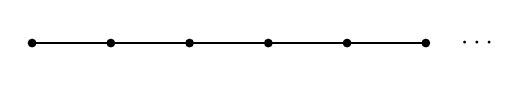
\begin{tikzpicture}[scale=1]
            \foreach \x in {0,1,2,3,4,5}{
                \fill (\x,0) circle (1.6pt);
            }
            \foreach \x in {0,1,2,3,4}{
                \draw (\x,0)--(\x+1,0);
            }
            \node at (5.65,0) {\(\cdots\)};
        \end{tikzpicture}
    \]
    Il primo vertice ha valenza \(1\), mentre tutti gli altri hanno valenza \(2\). Quindi esiste un solo vertice di valenza dispari.
\end{snippetsolution}

\section{Passeggiate, sentieri e cammini}

\begin{snippetdefinition}{Passeggiata}
    Dato un grafo \(G\), una \emph{passeggiata} è una successione finita alternata di vertici e lati
    \[
        v_0,e_1,v_1,e_2,v_2,\ldots,e_n,v_n
    \]
    tale che, per ogni \(i=1,\ldots,n\), gli estremi del lato \(e_i\) siano \(v_{i-1}\) e \(v_i\).

    I vertici \(v_0\) e \(v_n\) sono detti rispettivamente \emph{origine} e \emph{termine} della passeggiata.
\end{snippetdefinition}

\begin{snippetdefinition}{Sentiero}
    Un \emph{sentiero} è una passeggiata senza lati ripetuti. I vertici, invece, possono ripetersi.
\end{snippetdefinition}

\begin{snippetdefinition}{Cammino e circuito}
    Un \emph{cammino} è una passeggiata senza vertici ripetuti.

    Se l'unico vertice ripetuto è quello iniziale e finale, cioè se
    \[
        v_0=v_n,
    \]
    allora si parla di \emph{circuito}.
\end{snippetdefinition}

\[
    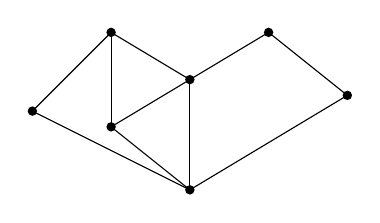
\begin{tikzpicture}[scale=1]
        \coordinate (a) at (-2,0);
        \coordinate (b) at (-1,1);
        \coordinate (c) at (0,0.4);
        \coordinate (d) at (1,1);
        \coordinate (e) at (2,0.2);
        \coordinate (f) at (0,-1);
        \coordinate (g) at (-1,-0.2);

        \draw (a)--(b)--(c)--(d)--(e)--(f)--(a);
        \draw (g)--(b);
        \draw (g)--(c);
        \draw (g)--(f);
        \draw (c)--(f);

        \foreach \p in {a,b,c,d,e,f,g}{
            \fill (\p) circle (1.7pt);
        }
    \end{tikzpicture}
\]

\begin{snippetdefinition}{Vertici connessi}
    Due vertici \(u,v\) di un grafo \(G\) si dicono \emph{connessi} se esiste una passeggiata che ha origine \(u\) e termine \(v\).

    Si ammette anche la passeggiata vuota, per cui ogni vertice è connesso con sé stesso.
\end{snippetdefinition}

\begin{snippetproposition}{Da passeggiata a cammino}
    Se due vertici \(u\) e \(v\) sono connessi, allora esiste un cammino che li congiunge.
\end{snippetproposition}

\begin{snippetproof}{}
    Sia
    \[
        v_0,e_1,v_1,\ldots,e_n,v_n
    \]
    una passeggiata da \(u=v_0\) a \(v=v_n\).

    Se nessun vertice si ripete, la passeggiata è già un cammino. Altrimenti esistono due indici \(i<j\) tali che
    \[
        v_i=v_j.
    \]
    Allora possiamo cancellare dalla passeggiata tutto il tratto compreso tra le due occorrenze di questo vertice:
    \[
        v_i,e_{i+1},v_{i+1},\ldots,e_j,v_j.
    \]
    Otteniamo ancora una passeggiata da \(u\) a \(v\), ma più corta.

    Ripetendo il procedimento, dopo un numero finito di passi non rimangono vertici ripetuti. La passeggiata ottenuta è quindi un cammino da \(u\) a \(v\).
\end{snippetproof}

\begin{snippetdefinition}{Lunghezza}
    La \emph{lunghezza} di una passeggiata è il numero di lati che compaiono nella passeggiata.

    In particolare, una passeggiata
    \[
        v_0,e_1,v_1,\ldots,e_n,v_n
    \]
    ha lunghezza \(n\).
\end{snippetdefinition}

\begin{snippetdefinition}{Distanza}
    La \emph{distanza} tra due vertici connessi \(u\) e \(v\), indicata con
    \[
        d(u,v),
    \]
    è la minima lunghezza di una passeggiata che congiunge \(u\) e \(v\).

    Ogni passeggiata di lunghezza minima è necessariamente un cammino.
\end{snippetdefinition}

\begin{snippetdefinition}{Grafo connesso}
    Un grafo \(G\) si dice \emph{connesso} se, per ogni coppia di vertici \(u,v\in V(G)\), esiste una passeggiata che congiunge \(u\) e \(v\).
\end{snippetdefinition}

La relazione di connessione tra vertici è una relazione di equivalenza. Le classi di equivalenza sono dette \emph{componenti connesse} del grafo.

\begin{snippetdefinition}{Componenti connesse}
    Le \emph{componenti connesse} di un grafo \(G\) sono i sottografi connessi massimali di \(G\), cioè i sottografi connessi che non sono contenuti propriamente in un sottografo connesso più grande.
\end{snippetdefinition}

\section{Cammini euleriani}

\begin{snippetdefinition}{Circuito euleriano}
    Sia \(G\) un grafo finito connesso. Un \emph{circuito euleriano} di \(G\) è una passeggiata chiusa, cioè con origine e termine uguali, che attraversa ogni lato di \(G\) esattamente una volta.

    I vertici possono essere ripetuti.
\end{snippetdefinition}

Il problema dei ponti di Königsberg chiede precisamente se il grafo associato ai ponti ammetta un circuito euleriano.

\begin{snippettheorem}{Teorema di Eulero}
    Sia \(G\) un grafo finito connesso. Allora \(G\) ammette un circuito euleriano se e solo se ogni vertice di \(G\) ha valenza pari.
\end{snippettheorem}

\begin{snippetproof}{}
    Dimostriamo le due implicazioni.

    \begin{iffproof}
        \item Supponiamo che esista un circuito euleriano
        \[
            v_0,e_1,v_1,e_2,\ldots,e_n,v_n,
            \qquad
            v_n=v_0.
        \]
        Ogni volta che la passeggiata passa per un vertice, usa un lato per entrare e un lato per uscire. Quindi i lati incidenti a ciascun vertice vengono accoppiati a due a due.

        Anche per il vertice iniziale \(v_0=v_n\) vale lo stesso ragionamento: c'è il primo lato con cui si esce e l'ultimo lato con cui si rientra. Dunque ogni vertice ha valenza pari.

        \item Supponiamo ora che tutti i vertici di \(G\) abbiano valenza pari.

        Partiamo da un vertice qualsiasi \(v_0\) e percorriamo lati non ancora usati, scegliendo ogni volta un lato disponibile. Siccome il grafo è finito, questo procedimento prima o poi si arresta.

        Mostriamo che può arrestarsi solo tornando al vertice iniziale \(v_0\). Infatti, se arriviamo a un vertice diverso da \(v_0\), abbiamo usato un lato per entrare. Poiché la valenza del vertice è pari, i lati incidenti non possono essere stati tutti usati: ogni volta che passiamo per quel vertice diverso da \(v_0\), i lati usati si accoppiano come uno di entrata e uno di uscita. Quindi non possiamo rimanere bloccati in un vertice diverso da \(v_0\).

        Otteniamo dunque un circuito chiuso \(C\).

        Se \(C\) contiene tutti i lati di \(G\), abbiamo finito. Altrimenti, poiché \(G\) è connesso, esiste un vertice di \(C\) incidente a qualche lato non ancora usato. Partendo da tale vertice e usando solo lati non ancora usati, per lo stesso ragionamento costruiamo un nuovo circuito chiuso. Inserendo questo circuito nel precedente, otteniamo un circuito chiuso più lungo.

        Ripetendo il procedimento, poiché il grafo è finito, alla fine otteniamo un circuito chiuso che contiene tutti i lati di \(G\). Questo è un circuito euleriano.
    \end{iffproof}
\end{snippetproof}

\begin{snippetcorollary}{Il problema dei ponti di Königsberg}
    Il grafo dei ponti di Königsberg non ammette un circuito euleriano.
\end{snippetcorollary}

\begin{snippetproof}{}
    Nel grafo dei ponti di Königsberg le quattro regioni hanno valenze
    \[
        3,\ 3,\ 3,\ 5.
    \]
    Sono quindi tutte dispari. Per il teorema di Eulero, non può esistere un circuito euleriano.
\end{snippetproof}

\begin{snippetdefinition}{Cammino euleriano aperto}
    Sia \(G\) un grafo finito connesso. Un \emph{cammino euleriano aperto} è una passeggiata che attraversa ogni lato di \(G\) esattamente una volta, ma la cui origine e il cui termine sono distinti.
\end{snippetdefinition}

\begin{snippettheorem}{Cammini euleriani aperti}
    Sia \(G\) un grafo finito connesso. Esiste un cammino euleriano aperto con origine e termine distinti se e solo se \(G\) ha esattamente due vertici di valenza dispari.

    In tal caso, i due vertici di valenza dispari sono necessariamente l'origine e il termine del cammino.
\end{snippettheorem}

\begin{snippetproof}{}
    Supponiamo che esista un cammino euleriano aperto da \(u\) a \(v\), con \(u\neq v\). Ogni vertice intermedio viene attraversato entrando e uscendo lo stesso numero di volte, quindi ha valenza pari. Invece \(u\) ha un'uscita in più rispetto alle entrate e \(v\) ha un'entrata in più rispetto alle uscite. Quindi \(u\) e \(v\) hanno valenza dispari, e tutti gli altri vertici hanno valenza pari.

    Viceversa, supponiamo che \(G\) abbia esattamente due vertici di valenza dispari, diciamo \(u\) e \(v\). Aggiungiamo un nuovo lato \(e\) che congiunge \(u\) e \(v\). Nel grafo così ottenuto ogni vertice ha valenza pari.

    Per il teorema di Eulero, il nuovo grafo ammette un circuito euleriano. Eliminando da tale circuito il lato aggiunto \(e\), rimane una passeggiata che attraversa ogni lato originario esattamente una volta, con origine \(u\) e termine \(v\). Dunque \(G\) ammette un cammino euleriano aperto.
\end{snippetproof}

\section{Alberi}

\begin{snippetdefinition}{Albero}
    Un \emph{albero} è un grafo connesso in cui non esistono cammini semplici chiusi, salvo i cammini banali.

    Equivalentemente, un albero è un grafo connesso e privo di circuiti.
\end{snippetdefinition}

\[
    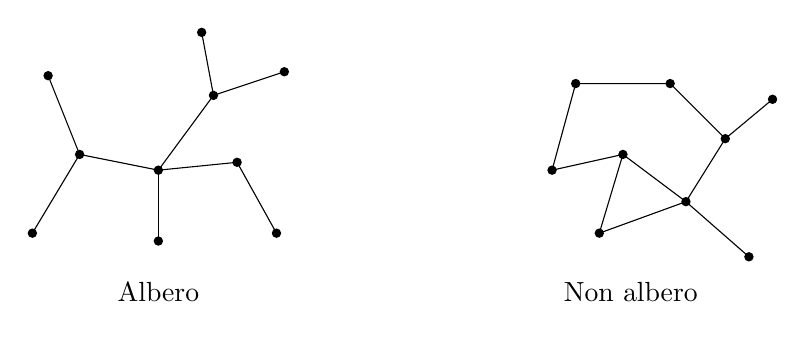
\begin{tikzpicture}[scale=1]
        % Albero
        \begin{scope}
            \node at (0,-1.55) {Albero};

            \coordinate (a) at (0,0);
            \coordinate (b) at (-1,0.2);
            \coordinate (c) at (-1.4,1.2);
            \coordinate (d) at (-1.6,-0.8);
            \coordinate (e) at (0,-0.9);
            \coordinate (f) at (1,0.1);
            \coordinate (g) at (1.5,-0.8);
            \coordinate (h) at (0.7,0.95);
            \coordinate (i) at (1.6,1.25);
            \coordinate (j) at (0.55,1.75);

            \draw (a)--(b)--(c);
            \draw (b)--(d);
            \draw (a)--(e);
            \draw (a)--(f)--(g);
            \draw (a)--(h)--(i);
            \draw (h)--(j);

            \foreach \p in {a,b,c,d,e,f,g,h,i,j}{
                \fill (\p) circle (1.7pt);
            }
        \end{scope}

        % Non albero
        \begin{scope}[xshift=6cm]
            \node at (0,-1.55) {Non albero};

            \coordinate (a) at (-1,0);
            \coordinate (b) at (-0.7,1.1);
            \coordinate (c) at (0.5,1.1);
            \coordinate (d) at (1.2,0.4);
            \coordinate (e) at (0.7,-0.4);
            \coordinate (f) at (-0.1,0.2);
            \coordinate (g) at (-0.4,-0.8);
            \coordinate (h) at (1.8,0.9);
            \coordinate (i) at (1.5,-1.1);

            \draw (a)--(b)--(c)--(d)--(e)--(f)--(a);
            \draw (f)--(g)--(e);
            \draw (d)--(h);
            \draw (e)--(i);

            \foreach \p in {a,b,c,d,e,f,g,h,i}{
                \fill (\p) circle (1.7pt);
            }
        \end{scope}
    \end{tikzpicture}
\]

In particolare, ogni albero è un grafo semplice. Il viceversa non è vero: un grafo semplice può contenere circuiti, e quindi non essere un albero.

\begin{snippetproposition}{Numero finito di lati}
    In un grafo semplice con un numero finito di vertici anche il numero di lati è finito.
\end{snippetproposition}

\begin{snippetproof}{}
    Sia \(G\) un grafo semplice con \(n\) vertici. Poiché il grafo è semplice, fra due vertici distinti può esserci al più un lato e non ci sono cappi.

    Ogni lato è quindi determinato da una coppia non ordinata di vertici distinti. Il numero massimo possibile di lati è
    \[
        \binom{n}{2}=\frac{n(n-1)}{2}.
    \]
    In particolare, \(G\) ha un numero finito di lati.
\end{snippetproof}

\begin{snippetcorollary}{}
    Ogni albero finito ha un numero finito di lati.
\end{snippetcorollary}

\begin{snippetproposition}{Foglie in un albero finito}
    In un albero finito con almeno due vertici ci sono almeno due vertici di valenza \(1\).
\end{snippetproposition}

\begin{snippetproof}{Idea della dimostrazione}
    Prendiamo un cammino semplice di lunghezza massima possibile:
    \[
        v_0,v_1,\ldots,v_k.
    \]
    Mostriamo che gli estremi \(v_0\) e \(v_k\) hanno valenza \(1\).

    Supponiamo, per esempio, che \(v_0\) abbia un vicino \(w\neq v_1\). Se \(w\) non appartenesse al cammino, allora potremmo estendere il cammino:
    \[
        w,v_0,v_1,\ldots,v_k,
    \]
    contraddicendo la massimalità della lunghezza.

    Se invece \(w\) appartenesse già al cammino, allora si formerebbe un circuito, impossibile perché il grafo è un albero.

    Quindi \(v_0\) ha come unico vicino \(v_1\), cioè ha valenza \(1\). Lo stesso ragionamento vale per \(v_k\).
\end{snippetproof}

\begin{snippetdefinition}{Foglia}
    Un vertice di valenza \(1\) si chiama \emph{foglia}.
\end{snippetdefinition}

\begin{snippettheorem}{Caratterizzazione degli alberi finiti tramite il numero di lati}
    Sia \(G\) un grafo connesso con \(n\) vertici. Allora \(G\) è un albero se e solo se ha \(n-1\) lati.
\end{snippettheorem}

\begin{snippetproof}{}
    Dimostriamo le due implicazioni.

    \begin{iffproof}
        \item Supponiamo che \(G\) sia un albero. Procediamo per induzione sul numero \(n\) di vertici.

        Se \(n=1\), allora \(G\) non ha lati, quindi ha
        \[
            0=n-1
        \]
        lati.

        Sia ora \(n>1\). Per la proposizione precedente, \(G\) ha almeno una foglia \(v\). Sia \(e\) l'unico lato incidente a \(v\). Consideriamo il grafo \(G'\) ottenuto da \(G\) cancellando il vertice \(v\) e il lato \(e\).

        Mostriamo che \(G'\) è ancora un albero. Certamente \(G'\) non contiene circuiti, perché un circuito in \(G'\) sarebbe anche un circuito in \(G\).

        Resta da osservare che \(G'\) è connesso. Presi due vertici \(u,w\in V(G')\), in \(G\) esiste un cammino che li congiunge. Tale cammino non può passare per \(v\), perché \(v\) è una foglia: se un cammino passasse per \(v\) come vertice interno, dovrebbe usare due lati incidenti a \(v\), ma \(v\) ha valenza \(1\). Quindi il cammino è interamente contenuto in \(G'\).

        Dunque \(G'\) è un albero con \(n-1\) vertici. Per ipotesi induttiva, \(G'\) ha
        \[
            (n-1)-1=n-2
        \]
        lati. Riaggiungendo il lato \(e\), otteniamo che \(G\) ha
        \[
            n-2+1=n-1
        \]
        lati.

        \item Supponiamo ora che \(G\) sia connesso con \(n\) vertici e \(n-1\) lati. Vogliamo mostrare che \(G\) non contiene circuiti.

        Per assurdo, supponiamo che \(G\) contenga un circuito. Eliminando un lato di tale circuito, il grafo resta connesso: infatti i due estremi del lato eliminato rimangono collegati dal resto del circuito. Quindi il lato eliminato non era necessario per la connessione.

        Se il nuovo grafo contiene ancora un circuito, possiamo ripetere il procedimento. Poiché il numero di lati è finito, dopo un numero finito di passi arriviamo a un grafo connesso senza circuiti, cioè a un albero \(T\), con gli stessi \(n\) vertici ma con meno di \(n-1\) lati.

        Questo è impossibile, perché abbiamo appena dimostrato che un albero con \(n\) vertici ha esattamente \(n-1\) lati.

        Quindi \(G\) non contiene circuiti. Essendo connesso, \(G\) è un albero.
    \end{iffproof}
\end{snippetproof}

\begin{snippetproposition}{Unicità dei cammini negli alberi}
    Un grafo \(G\) è un albero se e solo se, per ogni coppia di vertici distinti \(u,v\in V(G)\), esiste un unico cammino semplice che congiunge \(u\) e \(v\).
\end{snippetproposition}

\begin{snippetproof}{}
    \begin{iffproof}
        \item Supponiamo che \(G\) sia un albero. Poiché \(G\) è connesso, per ogni coppia di vertici distinti \(u,v\) esiste almeno un cammino che li congiunge.

        Mostriamo che tale cammino è unico. Se esistessero due cammini semplici distinti da \(u\) a \(v\), allora, seguendo il primo cammino da \(u\) a \(v\) e poi tornando da \(v\) a \(u\) lungo il secondo, si otterrebbe un cammino chiuso. Eliminando eventualmente le ripetizioni, si troverebbe un circuito, assurdo perché \(G\) è un albero.

        \item Viceversa, supponiamo che tra ogni coppia di vertici distinti esista un unico cammino semplice.

        Allora \(G\) è connesso, perché tra ogni coppia di vertici esiste un cammino. Inoltre \(G\) non può contenere circuiti: infatti, se ci fosse un circuito, presi due vertici distinti del circuito, potremmo congiungerli seguendo il circuito in due versi diversi, ottenendo due cammini semplici distinti.

        Quindi \(G\) è connesso e privo di circuiti, cioè è un albero.
    \end{iffproof}
\end{snippetproof}

\begin{snippetexercise}{Conteggio degli alberi piccoli}
    Dato l'insieme di vertici \(\{1,2,\ldots,n\}\), quanti alberi esistono con questo insieme di vertici?

    Per i primi valori di \(n\) si ottiene:
    \[
        \begin{array}{c|c}
            n & \text{numero di alberi etichettati} \\
            \hline
            1 & 1 \\
            2 & 1 \\
            3 & 3
        \end{array}
    \]

    Per \(n=3\), gli alberi possibili sono
    \[
        \begin{tikzpicture}[scale=0.9,baseline={(current bounding box.center)}]
            % tree 123
            \begin{scope}
                \coordinate (a) at (0,0);
                \coordinate (b) at (1,0);
                \coordinate (c) at (2,0);
                \draw (a)--(b)--(c);
                \foreach \p/\lab in {a/1,b/2,c/3}{
                    \fill (\p) circle (1.6pt);
                    \node[above] at (\p) {\(\lab\)};
                }
            \end{scope}

            % tree 132
            \begin{scope}[xshift=4cm]
                \coordinate (a) at (0,0);
                \coordinate (b) at (1,0);
                \coordinate (c) at (2,0);
                \draw (a)--(b)--(c);
                \foreach \p/\lab in {a/1,b/3,c/2}{
                    \fill (\p) circle (1.6pt);
                    \node[above] at (\p) {\(\lab\)};
                }
            \end{scope}

            % star centered at 1
            \begin{scope}[xshift=8cm]
                \coordinate (a) at (0,0);
                \coordinate (b) at (1,0.5);
                \coordinate (c) at (1,-0.5);
                \draw (a)--(b);
                \draw (a)--(c);
                \foreach \p/\lab in {a/1,b/2,c/3}{
                    \fill (\p) circle (1.6pt);
                    \node[above] at (\p) {\(\lab\)};
                }
            \end{scope}
        \end{tikzpicture}
    \]
    Questi tre alberi sono isomorfi come grafi non etichettati, ma sono distinti come alberi etichettati.
\end{snippetexercise}

\begin{snippetexercise}{Caso \(n=4\)}
    Dimostrare che il numero di alberi etichettati con insieme di vertici \(\{1,2,3,4\}\) è \(16\).

    Questo è il primo caso non banale della formula di Cayley:
    \[
        n^{n-2}=4^2=16.
    \]
\end{snippetexercise}

\section{Grafi planari}

\begin{snippetdefinition}{Grafo planare}
    Un grafo finito si dice \emph{planare} se può essere rappresentato nel piano nel modo seguente:
    \begin{itemize}
        \item i vertici sono rappresentati da punti del piano;
        \item i lati sono rappresentati da archi che congiungono i punti corrispondenti ai loro estremi;
        \item due archi non si intersecano, se non eventualmente nei loro estremi comuni.
    \end{itemize}
\end{snippetdefinition}

Per \emph{arco} si intende una curva continua che parametrizza un segmento topologico del piano. Nel caso dei cappi si ammette che il punto iniziale e il punto finale coincidano.

\[
    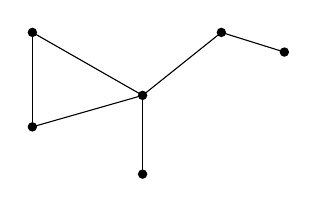
\begin{tikzpicture}[scale=1]
        \coordinate (a) at (0,0);
        \coordinate (b) at (0,1.2);
        \coordinate (c) at (1.4,0.4);
        \coordinate (d) at (1.4,-0.6);
        \coordinate (e) at (2.4,1.2);
        \coordinate (f) at (3.2,0.95);

        \draw (a)--(b);
        \draw (b)--(c);
        \draw (a)--(c);
        \draw (c)--(d);
        \draw (c)--(e);
        \draw (e)--(f);

        \foreach \p in {a,b,c,d,e,f}{
            \fill (\p) circle (1.7pt);
        }
    \end{tikzpicture}
\]

Bisogna distinguere tra il grafo astratto e una sua rappresentazione nel piano. Un grafo planare può essere disegnato anche in modo non planare, cioè con incroci tra lati. La presenza di incroci in un disegno non dimostra che il grafo non sia planare.

\[
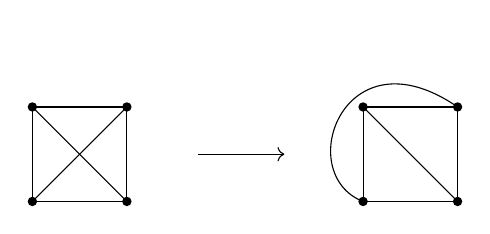
\begin{tikzpicture}[scale=1]
    % Disegno con incrocio di K_4
    \begin{scope}
        \coordinate (a) at (0,0);
        \coordinate (b) at (1.2,0);
        \coordinate (c) at (1.2,1.2);
        \coordinate (d) at (0,1.2);

        \draw (a)--(b)--(c)--(d)--cycle;
        \draw (a)--(c);
        \draw (b)--(d);

        \foreach \p in {a,b,c,d}{
            \fill (\p) circle (1.7pt);
        }
    \end{scope}

    \draw[->] (2.1,0.6)--(3.2,0.6);

    % Disegno planare di K_4
    \begin{scope}[xshift=4.2cm]
        \coordinate (a) at (0,0);
        \coordinate (b) at (1.2,0);
        \coordinate (c) at (1.2,1.2);
        \coordinate (d) at (0,1.2);

        \draw (a)--(b)--(c)--(d)--cycle;
        \draw (d)--(b);
        \draw (a) .. controls +(-0.90,0.35) and +(-1.45,1.00) .. (c);

        \foreach \p in {a,b,c,d}{
            \fill (\p) circle (1.7pt);
        }
    \end{scope}
\end{tikzpicture}
\]

\begin{snippetdefinition}{Facce}
    Una rappresentazione planare di un grafo planare divide il piano in regioni connesse, dette \emph{facce}. Tra queste si conta anche la faccia esterna, cioè la regione illimitata.
\end{snippetdefinition}

\begin{snippetexample}{Facce di una rappresentazione planare}
    Il seguente grafo planare ha \(4\) vertici, \(6\) lati e \(4\) facce.
    \[
        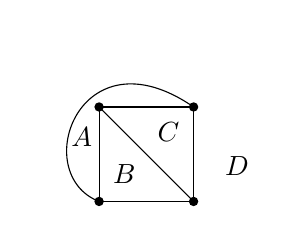
\begin{tikzpicture}[scale=1]
            \coordinate (a) at (0,0);
            \coordinate (b) at (1.2,0);
            \coordinate (c) at (1.2,1.2);
            \coordinate (d) at (0,1.2);

            \draw (a)--(b)--(c)--(d)--cycle;
            \draw (d)--(b);
            \draw (a) .. controls +(-0.90,0.35) and +(-1.45,1.00) .. (c);

            % Etichette delle regioni
            \node at (-0.22,0.82) {\(A\)};
            \node at (0.32,0.35) {\(B\)};
            \node at (0.88,0.88) {\(C\)};
            \node at (1.75,0.45) {\(D\)};

            \foreach \p in {a,b,c,d}{
                \fill (\p) circle (1.7pt);
            }
        \end{tikzpicture}
    \]
\end{snippetexample}

\begin{snippettheorem}{Formula di Eulero per grafi planari connessi}
    Sia \(G\) un grafo planare connesso, rappresentato nel piano. Indichiamo con
    \[
        v=\text{numero di vertici},
        \qquad
        l=\text{numero di lati},
        \qquad
        f=\text{numero di facce}.
    \]
    Allora
    \[
        v-l+f=2.
    \]
\end{snippettheorem}

\begin{snippetproof}{}
    Dimostriamo che la quantità
    \[
        v-l+f
    \]
    rimane invariata quando eliminiamo opportunamente lati appartenenti a circuiti, fino ad arrivare a un albero.

    Se \(G\) è un albero, allora
    \[
        l=v-1.
    \]
    Inoltre una rappresentazione planare di un albero non racchiude regioni limitate, quindi ha una sola faccia, quella esterna:
    \[
        f=1.
    \]
    Pertanto
    \[
        v-l+f
        =
        v-(v-1)+1
        =
        2.
    \]

    Supponiamo ora che \(G\) non sia un albero. Poiché \(G\) è connesso, allora contiene almeno un circuito. Scegliamo un lato \(e\) appartenente a un circuito e cancelliamolo.

    Il grafo ottenuto resta connesso, perché gli estremi di \(e\) sono ancora collegati dal resto del circuito. Il numero di vertici resta uguale, il numero di lati diminuisce di \(1\), e il numero di facce diminuisce di \(1\): cancellare un lato appartenente a un circuito fonde due facce adiacenti in una sola.

    Quindi la quantità
    \[
        v-l+f
    \]
    non cambia, infatti:
    \[
        v-(l-1)+(f-1)=v-l+f.
    \]

    Ripetendo il procedimento un numero finito di volte, arriviamo a un albero. Siccome per gli alberi la quantità vale \(2\), essa vale \(2\) anche per il grafo iniziale.
\end{snippetproof}

\section{Grafi completi}

\begin{snippetdefinition}{Grafo completo}
    Dato un insieme di \(n\) vertici, il \emph{grafo completo} \(K_n\) è il grafo semplice in cui ogni vertice è connesso a tutti gli altri.

    In particolare:
    \[
        v=n,
        \qquad
        l=\binom{n}{2}=\frac{n(n-1)}{2}.
    \]
\end{snippetdefinition}

Vedremo in seguito che \(K_5\) non è planare.

\section{Grafi planari, grafi completi e formula di Cayley}

Ricordiamo che, se un grafo planare connesso ha \(v\) vertici, \(l\) lati e \(f\) facce, contando anche la faccia illimitata, allora vale la formula di Eulero:
\[
    v-l+f=2.
\]

\begin{snippetdefinition}{Grafo completo}
    Dato un insieme di \(n\) vertici, il \emph{grafo completo} \(K_n\) è il grafo semplice in cui ogni vertice è connesso a tutti gli altri.

    Per tale grafo si ha
    \[
        v=n,
        \qquad
        l=\binom{n}{2}=\frac{n(n-1)}{2}.
    \]
\end{snippetdefinition}

Osserviamo che, per \(n\leq 4\), il grafo \(K_n\) è planare.

\[
\begin{tikzpicture}[scale=1]
    % K_1
    \begin{scope}
        \fill (0,0) circle (1.8pt);
        \node at (0,-0.45) {\(n=1\)};
    \end{scope}

    % K_2
    \begin{scope}[xshift=2.4cm]
        \coordinate (a) at (0,0);
        \coordinate (b) at (1,0);

        \draw (a)--(b);

        \fill (a) circle (1.8pt);
        \fill (b) circle (1.8pt);

        \node at (0.5,-0.45) {\(n=2\)};
    \end{scope}

    % K_3
    \begin{scope}[xshift=5cm]
        \coordinate (a) at (0,0);
        \coordinate (b) at (1,0);
        \coordinate (c) at (0.5,0.85);

        \draw (a)--(b)--(c)--cycle;

        \foreach \p in {a,b,c}{
            \fill (\p) circle (1.8pt);
        }

        \node at (0.5,-0.45) {\(n=3\)};
    \end{scope}

    % K_4
    \begin{scope}[xshift=8cm]
        \coordinate (a) at (0,0);
        \coordinate (b) at (1,0);
        \coordinate (c) at (1,1);
        \coordinate (d) at (0,1);

        \draw (a)--(b)--(c)--(d)--cycle;
        \draw (d)--(b);
        \draw (a) .. controls +(-0.75,0.30) and +(-1.05,0.75) .. (c);

        \foreach \p in {a,b,c,d}{
            \fill (\p) circle (1.8pt);
        }

        \node at (0.5,-0.45) {\(n=4\)};
    \end{scope}
\end{tikzpicture}
\]

\begin{snippetproposition}{Il grafo \(K_5\) non è planare}
    Il grafo completo \(K_5\) non è planare. Di conseguenza, \(K_n\) non è planare per ogni \(n\geq 5\).
\end{snippetproposition}

\begin{snippetproof}{}
    Supponiamo per assurdo che \(K_5\) sia planare. Allora
    \[
        v=5,
        \qquad
        l=\frac{5\cdot 4}{2}=10.
    \]
    Per la formula di Eulero avremmo
    \[
        5-10+f=2,
    \]
    da cui
    \[
        f=7.
    \]

    Poiché \(K_5\) è semplice, ogni faccia è delimitata da almeno \(3\) lati. Se sommiamo, su tutte le facce, il numero di lati che le delimitano, otteniamo almeno
    \[
        3f=21.
    \]
    D'altra parte ogni lato può delimitare al massimo due facce, quindi questa stessa somma è al più
    \[
        2l=20.
    \]
    Otteniamo quindi
    \[
        21\leq 20,
    \]
    che è assurdo.

    Quindi \(K_5\) non è planare.

    Infine, se \(n\geq 5\), allora \(K_n\) contiene un sottografo isomorfo a \(K_5\). Se \(K_n\) fosse planare, anche ogni suo sottografo sarebbe planare, in particolare \(K_5\), assurdo. Dunque \(K_n\) non è planare per ogni \(n\geq 5\).
\end{snippetproof}

\begin{snippetdefinition}{Grafo bipartito}
    Un grafo \(G\) si dice \emph{bipartito} se l'insieme dei suoi vertici può essere scritto come unione disgiunta
    \[
        V(G)=V_1\union V_2,
        \qquad
        V_1\intersection V_2=\emptyset,
    \]
    con \(V_1,V_2\neq\emptyset\), in modo tale che ogni lato unisca un vertice di \(V_1\) con un vertice di \(V_2\).

    In particolare, in un grafo bipartito non ci sono cappi e non esistono lati che congiungono due vertici appartenenti alla stessa parte.
\end{snippetdefinition}

\begin{snippetdefinition}{Grafo bipartito completo}
    Dati due interi positivi \(m,n\), il \emph{grafo bipartito completo} \(K_{m,n}\) è il grafo il cui insieme dei vertici è l'unione disgiunta di due insiemi
    \[
        V_1\union V_2,
        \qquad
        \cardinality{V_1}=m,
        \qquad
        \cardinality{V_2}=n,
    \]
    e il cui insieme dei lati è
    \[
        V_1\times V_2.
    \]
    Il lato \((P,Q)\), con \(P\in V_1\) e \(Q\in V_2\), ha estremi \(P\) e \(Q\).

    In particolare, \(K_{m,n}\) è un grafo semplice e ha
    \[
        v=m+n,
        \qquad
        l=mn.
    \]
\end{snippetdefinition}

\begin{snippetexample}{Il grafo \(K_{2,3}\)}
    Il grafo \(K_{2,3}\) è planare.

    \[
        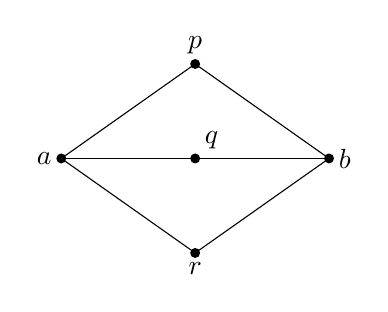
\begin{tikzpicture}[scale=1]
            \coordinate (a) at (-1.7,0);
            \coordinate (b) at (1.7,0);
            \coordinate (p) at (0,1.2);
            \coordinate (q) at (0,0);
            \coordinate (r) at (0,-1.2);

            \draw (a)--(p)--(b);
            \draw (a)--(q)--(b);
            \draw (a)--(r)--(b);

            \foreach \x in {a,b,p,q,r}{
                \fill (\x) circle (1.8pt);
            }

            \node[left] at (a) {\(a\)};
            \node[right] at (b) {\(b\)};
            \node[above] at (p) {\(p\)};
            \node[above right] at (q) {\(q\)};
            \node[below] at (r) {\(r\)};
        \end{tikzpicture}
    \]

    Le due parti della bipartizione sono
    \[
        V_1=\{a,b\},
        \qquad
        V_2=\{p,q,r\}.
    \]
\end{snippetexample}

\begin{snippetproposition}{Il grafo \(K_{3,3}\) non è planare}
    Il grafo bipartito completo \(K_{3,3}\) non è planare.
\end{snippetproposition}

\begin{snippetproof}{}
    Supponiamo per assurdo che \(K_{3,3}\) sia planare. Allora
    \[
        v=6,
        \qquad
        l=9.
    \]
    Per la formula di Eulero avremmo
    \[
        6-9+f=2,
    \]
    quindi
    \[
        f=5.
    \]

    Mostriamo che ogni faccia deve essere delimitata da almeno \(4\) lati. Infatti, se una faccia fosse delimitata da \(3\) lati, allora i tre vertici coinvolti formerebbero un triangolo. Ma in un grafo bipartito non possono esistere triangoli, perché tra tre vertici almeno due stanno nella stessa parte della bipartizione e quindi non sono connessi da un lato.

    Quindi, sommando i lati che delimitano le facce, otteniamo almeno
    \[
        4f=20.
    \]
    D'altra parte ogni lato delimita al massimo due facce, perciò tale somma è al più
    \[
        2l=18.
    \]
    Segue
    \[
        20\leq 18,
    \]
    che è assurdo.

    Pertanto \(K_{3,3}\) non è planare.
\end{snippetproof}

\begin{snippettheorem}{Teorema di Kuratowski}
    Un grafo finito è non planare se e solo se contiene una suddivisione di \(K_5\) oppure una suddivisione di \(K_{3,3}\).

    Qui ``contiene'' significa che il grafo contiene come sottografo un grafo ottenuto da \(K_5\) o da \(K_{3,3}\) suddividendo alcuni lati, cioè sostituendo certi lati con cammini i cui vertici interni sono nuovi.
\end{snippettheorem}

\section{Formula di Cayley e codice di Prüfer}

Vogliamo ora contare gli alberi etichettati con \(n\) vertici.

\begin{snippettheorem}{Formula di Cayley}
    Esistono esattamente
    \[
        n^{n-2}
    \]
    alberi etichettati con insieme dei vertici \(\{1,\ldots,n\}\).
\end{snippettheorem}

Per dimostrare la formula di Cayley useremo il codice di Prüfer, che associa a ogni albero etichettato una sequenza di lunghezza \(n-2\) a valori in \(\{1,\ldots,n\}\).

Sia quindi \(T\) un albero con \(n\geq 2\) vertici, etichettati con i numeri
\[
    1,2,\ldots,n.
\]
Più in generale, basterebbe avere un insieme di etichette totalmente ordinato.

\begin{snippetdefinition}{Sequenze associate a un albero}
    Poniamo
    \[
        T_0=T.
    \]
    Costruiamo iterativamente tre sequenze:
    \[
        x_1,\ldots,x_{n-1},
        \qquad
        y_1,\ldots,y_{n-1},
        \qquad
        T_1,\ldots,T_{n-1}.
    \]

    Al primo passo:
    \begin{itemize}
        \item \(x_1\) è il più piccolo vertice di valenza \(1\) in \(T_0\);
        \item \(y_1\) è l'unico vertice adiacente a \(x_1\);
        \item \(T_1\) è l'albero ottenuto da \(T_0\) cancellando \(x_1\) e il lato che congiunge \(x_1\) a \(y_1\).
    \end{itemize}

    Poi si procede nello stesso modo su \(T_1\), poi su \(T_2\), e così via, finché resta un solo vertice.
\end{snippetdefinition}

\begin{snippetexample}{Calcolo del codice di Prüfer}
    Consideriamo l'albero seguente.

    \[
        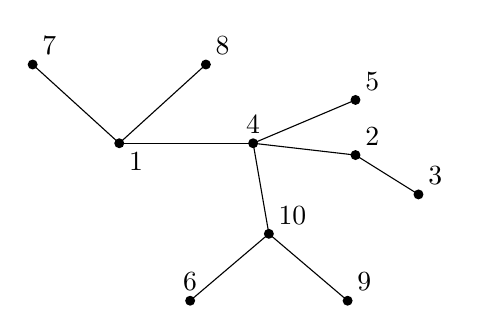
\begin{tikzpicture}[scale=1]
            \coordinate (v1) at (0,0);
            \coordinate (v7) at (-1.1,1);
            \coordinate (v8) at (1.1,1);
            \coordinate (v4) at (1.7,0);
            \coordinate (v5) at (3,0.55);
            \coordinate (v2) at (3,-0.15);
            \coordinate (v3) at (3.8,-0.65);
            \coordinate (v10) at (1.9,-1.15);
            \coordinate (v6) at (0.9,-2);
            \coordinate (v9) at (2.9,-2);

            \draw (v1)--(v7);
            \draw (v1)--(v8);
            \draw (v1)--(v4);
            \draw (v4)--(v5);
            \draw (v4)--(v2);
            \draw (v2)--(v3);
            \draw (v4)--(v10);
            \draw (v10)--(v6);
            \draw (v10)--(v9);

            \fill (v1) circle (1.8pt);
            \node[below right] at (v1) {\(1\)};
            \fill (v2) circle (1.8pt);
            \node[above right] at (v2) {\(2\)};
            \fill (v3) circle (1.8pt);
            \node[above right] at (v3) {\(3\)};
            \fill (v4) circle (1.8pt);
            \node[above] at (v4) {\(4\)};
            \fill (v5) circle (1.8pt);
            \node[above right] at (v5) {\(5\)};
            \fill (v6) circle (1.8pt);
            \node[above] at (v6) {\(6\)};
            \fill (v7) circle (1.8pt);
            \node[above right] at (v7) {\(7\)};
            \fill (v8) circle (1.8pt);
            \node[above right] at (v8) {\(8\)};
            \fill (v9) circle (1.8pt);
            \node[above right] at (v9) {\(9\)};
            \fill (v10) circle (1.8pt);
            \node[above right] at (v10) {\(10\)};
        \end{tikzpicture}
    \]

    Applichiamo l'algoritmo cancellando, a ogni passo, la foglia con etichetta minima. Si ottiene
    \[
        \begin{array}{c|ccccccccc}
            i   & 1 & 2 & 3 & 4  & 5 & 6 & 7 & 8  & 9  \\
            \hline
            x_i & 3 & 2 & 5 & 6  & 7 & 8 & 1 & 4  & 9  \\
            y_i & 2 & 4 & 4 & 10 & 1 & 1 & 4 & 10 & 10
        \end{array}
    \]
    La sequenza di Prüfer è formata dai primi \(n-2\) termini della sequenza \(y_i\), quindi in questo caso è
    \[
        (2,4,4,10,1,1,4,10).
    \]
\end{snippetexample}

\begin{snippetproposition}{Proprietà delle sequenze \(x_i\) e \(y_i\)}
    Con la costruzione precedente valgono le seguenti proprietà.
    \begin{enumerate}
        \item Nella sequenza \(x_1,\ldots,x_{n-1}\) compaiono tutti i vertici da \(1\) a \(n-1\), ciascuno una sola volta.
        \item Le coppie \((x_i,y_i)\) sono esattamente gli estremi degli \(n-1\) lati dell'albero.
        \item Per ogni vertice \(a\), la valenza di \(a\) in \(T\) è uguale al numero di volte in cui \(a\) compare complessivamente nella sequenza
        \[
            x_1,\ldots,x_{n-1},y_1,\ldots,y_{n-1}.
        \]
        \item Si ha necessariamente
        \[
            y_{n-1}=n.
        \]
    \end{enumerate}
\end{snippetproposition}

\begin{snippetproof}{}
    Un vertice, una volta cancellato, non può più ricomparire nella sequenza \(x_i\). Inoltre, finché un albero ha almeno due vertici, esso possiede almeno due foglie. Dal momento che cancelliamo sempre la foglia con etichetta minima, il vertice \(n\) non può mai essere scelto come \(x_i\) prima dell'ultimo vertice rimasto: se \(n\) fosse una foglia, esisterebbe comunque un'altra foglia con etichetta minore.

    Quindi i vertici cancellati sono precisamente \(1,\ldots,n-1\), ciascuno una sola volta.

    Al passo \(i\) cancelliamo esattamente il lato che congiunge \(x_i\) a \(y_i\). Quindi le coppie \((x_i,y_i)\) registrano tutti e soli i lati dell'albero.

    La valenza di un vertice è il numero di lati incidenti a quel vertice. Poiché i lati sono descritti dalle coppie \((x_i,y_i)\), la valenza di un vertice coincide con il numero totale delle sue occorrenze nelle due sequenze \(x_i\) e \(y_i\).

    Infine, poiché il vertice \(n\) è l'ultimo sopravvissuto, nell'ultimo passo il lato cancellato ha l'altro estremo uguale a \(n\). Dunque
    \[
        y_{n-1}=n.
    \]
\end{snippetproof}

\begin{snippetdefinition}{Codice di Prüfer}
    Il \emph{codice di Prüfer} di un albero etichettato con vertici \(\{1,\ldots,n\}\) è la sequenza
    \[
        (y_1,y_2,\ldots,y_{n-2})\in \{1,\ldots,n\}^{n-2}
    \]
    ottenuta tramite l'algoritmo di cancellazione delle foglie.
\end{snippetdefinition}

Abbiamo quindi definito una funzione
\[
    \{\text{alberi etichettati con }n\text{ vertici}\}
    \longrightarrow
    \{1,\ldots,n\}^{n-2}.
\]
Poiché l'insieme di arrivo ha cardinalità \(n^{n-2}\), per dimostrare la formula di Cayley basta mostrare che questa funzione è biiettiva.

\begin{snippetproposition}{Ricostruzione di un albero dal codice di Prüfer}
    Ogni sequenza
    \[
        (y_1,\ldots,y_{n-2})\in\{1,\ldots,n\}^{n-2}
    \]
    è il codice di Prüfer di uno e un solo albero etichettato con vertici \(\{1,\ldots,n\}\).
\end{snippetproposition}

\begin{snippetproof}{}
    Partiamo da una sequenza arbitraria
    \[
        (y_1,\ldots,y_{n-2})\in\{1,\ldots,n\}^{n-2}.
    \]
    Per comodità poniamo
    \[
        y_{n-1}=n.
    \]

    Vogliamo ricostruire le sequenze \(x_1,\ldots,x_{n-1}\) e \(y_1,\ldots,y_{n-1}\), e quindi i lati dell'albero.

    Definiamo \(x_1\) come il più piccolo vertice che non compare nella sequenza
    \[
        (y_1,y_2,\ldots,y_{n-1}).
    \]
    Poi inseriamo il lato
    \[
        (x_1,y_1).
    \]

    Ricorsivamente, supponendo già definiti \(x_1,\ldots,x_{i-1}\), definiamo \(x_i\) come il più piccolo vertice che non compare nella sequenza
    \[
        (x_1,x_2,\ldots,x_{i-1},y_i,y_{i+1},\ldots,y_{n-1}).
    \]
    Aggiungiamo poi il lato
    \[
        (x_i,y_i).
    \]

    In questo modo la sequenza di partenza determina in modo univoco tutte le coppie
    \[
        (x_i,y_i),
        \qquad
        i=1,\ldots,n-1.
    \]
    Quindi, se il grafo ottenuto è effettivamente un albero, il codice di Prüfer determina univocamente l'albero. Questo mostra l'iniettività della costruzione inversa.

    Resta da verificare che, partendo da una sequenza arbitraria, il grafo costruito sia sempre un albero. Lo dimostriamo per induzione su \(n\).

    Se \(n=2\), la sequenza di Prüfer ha lunghezza \(0\), quindi è vuota. Poniamo
    \[
        y_1=2.
    \]
    Il più piccolo vertice che non compare nella sequenza è \(1\), quindi \(x_1=1\). Il grafo costruito ha vertici \(1,2\) e un unico lato che li congiunge. Dunque è un albero.

    Supponiamo ora \(n>2\) e assumiamo la tesi vera per \(n-1\). Applicando la costruzione alla sequenza data, otteniamo le sequenze
    \[
        x_1,\ldots,x_{n-1},
        \qquad
        y_1,\ldots,y_{n-1}.
    \]
    Consideriamo il grafo ottenuto ignorando il primo lato \((x_1,y_1)\) e il vertice \(x_1\). Esso ha vertici
    \[
        x_2,x_3,\ldots,x_{n-1},n
    \]
    e lati
    \[
        (x_i,y_i),
        \qquad
        i=2,\ldots,n-1.
    \]
    Per ipotesi induttiva questo grafo è un albero. In particolare è connesso, ha \(n-1\) vertici e \(n-2\) lati.

    Il grafo completo costruito dalla sequenza contiene inoltre il vertice \(x_1\) e il lato \((x_1,y_1)\). Per definizione di \(x_1\), il vertice \(x_1\) non compare tra \(y_1,\ldots,y_{n-1}\), quindi \(x_1\) viene aggiunto come foglia. Ne segue che il grafo resta connesso e non si crea alcun circuito.

    Quindi il grafo costruito ha \(n\) vertici, \(n-1\) lati ed è connesso; pertanto è un albero.
\end{snippetproof}

\begin{snippetproof}{Dimostrazione della formula di Cayley}
    Il codice di Prüfer definisce una corrispondenza biunivoca tra gli alberi etichettati con vertici \(\{1,\ldots,n\}\) e le sequenze di lunghezza \(n-2\) a valori in \(\{1,\ldots,n\}\).

    Il numero di tali sequenze è
    \[
        \underbrace{n\cdot n\cdots n}_{n-2\text{ volte}}=n^{n-2}.
    \]
    Dunque il numero di alberi etichettati con \(n\) vertici è
    \[
        n^{n-2}.
    \]
\end{snippetproof}

\section{Alberi generatori e grafi di Cayley}

\begin{snippetdefinition}{Albero, sottoalbero e albero generatore}
    Ricordiamo che un \emph{albero} è un grafo connesso e senza circuiti. Un \emph{sottoalbero} di un grafo \(G\) è un sottografo di \(G\) che è un albero.

    Sia \(G\) un grafo connesso. Un \emph{albero generatore} di \(G\) è un sottoalbero \(T\) di \(G\) tale che
    \[
        V(T)=V(G).
    \]
    Cioè \(T\) contiene tutti i vertici di \(G\), ma non necessariamente tutti i lati di \(G\).
\end{snippetdefinition}

\begin{snippetexample}{Alberi generatori}
    Un grafo connesso può ammettere più alberi generatori.
    \[
    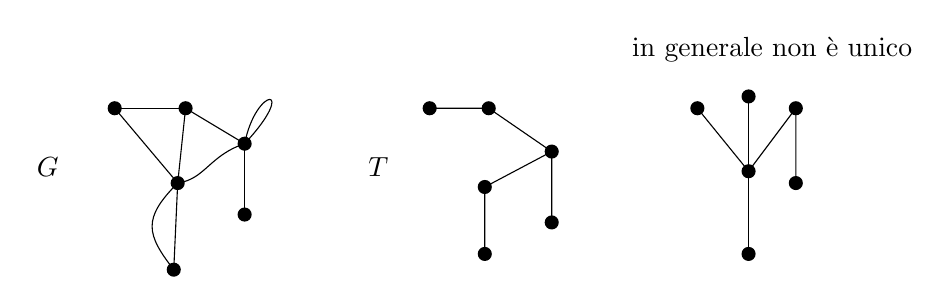
\begin{tikzpicture}[
        scale=1,
        line cap=round,
        line join=round,
        v/.style={circle, fill, inner sep=1.8pt}
    ]
        % Primo grafo: G
        \begin{scope}
            \node at (-0.85,0.25) {\(G\)};

            \coordinate (g1) at (0,1);
            \coordinate (g2) at (0.9,1);
            \coordinate (g3) at (0.8,0.05);
            \coordinate (g4) at (1.65,0.55);
            \coordinate (g5) at (1.65,-0.35);
            \coordinate (g6) at (0.75,-1.05);

            \draw (g1)--(g2);
            \draw (g1)--(g3);
            \draw (g2)--(g3);
            \draw (g2)--(g4);
            \draw (g3) .. controls +(0.35,0.05) and +(-0.45,-0.15) .. (g4);
            \draw (g4)--(g5);

            % doppia connessione verso il basso
            \draw (g3)--(g6);
            \draw (g3) .. controls +(-0.45,-0.45) and +(-0.35,0.45) .. (g6);

            % cappio
            \draw (g4) .. controls +(0.15,0.75) and +(0.70,0.75) .. (g4);

            \foreach \p in {g1,g2,g3,g4,g5,g6}{
                \node[v] at (\p) {};
            }
        \end{scope}

        % Secondo grafo: sottografo T
        \begin{scope}[xshift=4cm]
            \node at (-0.65,0.25) {\(T\)};

            \coordinate (t1) at (0,1);
            \coordinate (t2) at (0.75,1);
            \coordinate (t3) at (0.70,0);
            \coordinate (t4) at (1.55,0.45);
            \coordinate (t5) at (1.55,-0.45);
            \coordinate (t6) at (0.70,-0.85);

            \draw (t1)--(t2)--(t4)--(t5);
            \draw (t4)--(t3)--(t6);

            \foreach \p in {t1,t2,t3,t4,t5,t6}{
                \node[v] at (\p) {};
            }
        \end{scope}

        % Terzo grafo
        \begin{scope}[xshift=7.4cm]
            \node at (0.95,1.75) {in generale non è unico};

            \coordinate (u0) at (0.65,0.2);
            \coordinate (u1) at (0,1);
            \coordinate (u2) at (0.65,1.15);
            \coordinate (u3) at (1.25,1);
            \coordinate (u4) at (1.25,0.05);
            \coordinate (u5) at (0.65,-0.85);

            \draw (u1)--(u0);
            \draw (u2)--(u0);
            \draw (u0)--(u3)--(u4);
            \draw (u0)--(u5);

            \foreach \p in {u0,u1,u2,u3,u4,u5}{
                \node[v] at (\p) {};
            }
        \end{scope}
    \end{tikzpicture}
    \]
\end{snippetexample}

\begin{snippetdefinition}{Sottoalbero massimale}
    Sia \(G\) un grafo. Un sottoalbero \(T\) di \(G\) si dice \emph{massimale} se non esiste un sottoalbero \(T'\) di \(G\) tale che
    \[
        T \subsetneq T'.
    \]
    La massimalità è intesa rispetto all'inclusione di sottografi: si confrontano sia i vertici sia i lati.
\end{snippetdefinition}

\begin{snippetproposition}{Alberi generatori e sottoalberi massimali}
    Sia \(G\) un grafo connesso e sia \(T\) un sottoalbero di \(G\). Allora \(T\) è un albero generatore di \(G\) se e solo se \(T\) è massimale tra i sottoalberi di \(G\).
\end{snippetproposition}

\begin{snippetproof}{}
    Dimostriamo le due implicazioni.

    \begin{iffproof}
        \item Supponiamo che \(T\) sia un albero generatore di \(G\). Allora \(V(T)=V(G)\).

        Se, per assurdo, \(T\) non fosse massimale, esisterebbe un sottoalbero \(T'\) di \(G\) tale che
        \[
            T \subsetneq T'.
        \]
        Poiché \(T\) contiene già tutti i vertici di \(G\), il sottografo \(T'\) non può aggiungere nuovi vertici: deve quindi aggiungere almeno un lato \(uv\notin E(T)\).

        Gli estremi \(u\) e \(v\) appartengono a \(V(T)\). Siccome \(T\) è un albero, in \(T\) esiste un cammino che congiunge \(u\) e \(v\). Aggiungendo il lato \(uv\), questo cammino diventa un circuito. Quindi \(T'\) contiene un circuito e non può essere un albero, assurdo.

        Dunque \(T\) è massimale.

        \item Supponiamo ora che \(T\) sia massimale tra i sottoalberi di \(G\). Vogliamo mostrare che \(T\) contiene tutti i vertici di \(G\).

        Per assurdo, supponiamo che esista un vertice \(v\in V(G)\setminus V(T)\). Scegliamo un vertice \(u\in V(T)\). Poiché \(G\) è connesso, esiste un cammino in \(G\) che congiunge \(u\) a \(v\):
        \[
            u=x_0,x_1,\ldots,x_m=v.
        \]
        Sia \(i\) il primo indice tale che \(x_i\notin V(T)\). Allora \(x_{i-1}\in V(T)\) e il lato \(x_{i-1}x_i\) appartiene a \(G\).

        Aggiungiamo a \(T\) il nuovo vertice \(x_i\) e il lato \(x_{i-1}x_i\). Otteniamo un nuovo sottografo \(T'\) di \(G\), strettamente più grande di \(T\). Inoltre \(T'\) è ancora un albero, perché abbiamo aggiunto un nuovo vertice come foglia: il grafo resta connesso e non si crea alcun circuito.

        Questo contraddice la massimalità di \(T\). Quindi non esistono vertici di \(G\) fuori da \(T\), cioè
        \[
            V(T)=V(G).
        \]
        Dunque \(T\) è un albero generatore.
    \end{iffproof}
\end{snippetproof}

Vogliamo ora dimostrare che ogni grafo connesso ammette almeno un albero generatore. Per grafi finiti questo si può vedere rimuovendo lati dai circuiti finché non restano più circuiti. Per grafi infiniti useremo il lemma di Zorn.

\begin{snippettheorem}{Lemma di Zorn}
    Sia \(P\) un insieme non vuoto parzialmente ordinato. Se ogni sottoinsieme totalmente ordinato \(S\subseteq P\) ammette un maggiorante in \(P\), allora \(P\) contiene almeno un elemento massimale.
\end{snippettheorem}

\begin{snippettheorem}{Esistenza di alberi generatori}
    Ogni grafo connesso non vuoto \(G\) ammette un albero generatore.
\end{snippettheorem}

\begin{snippetproof}{}
    Consideriamo l'insieme
    \[
        P=\{T\mid T \text{ è un sottoalbero di }G\},
    \]
    ordinato per inclusione.

    L'insieme \(P\) è non vuoto: infatti, preso un vertice \(v\in V(G)\), il sottografo formato dal solo vertice \(v\) è un albero.

    Sia ora \(\mathcal{S}\subseteq P\) un sottoinsieme totalmente ordinato, cioè una catena di sottoalberi di \(G\). Vogliamo costruire un maggiorante di \(\mathcal{S}\) in \(P\).

    Definiamo \(T\) come l'unione di tutti i sottoalberi appartenenti a \(\mathcal{S}\):
    \[
        V(T)=\bigcup_{A\in\mathcal{S}} V(A),
        \qquad
        E(T)=\bigcup_{A\in\mathcal{S}} E(A).
    \]
    Allora \(T\) è un sottografo di \(G\) e contiene ogni elemento di \(\mathcal{S}\). Mostriamo che \(T\) è un albero.

    Prima di tutto, \(T\) è connesso. Se \(u,v\in V(T)\), allora esistono \(T_1,T_2\in\mathcal{S}\) tali che
    \[
        u\in V(T_1),
        \qquad
        v\in V(T_2).
    \]
    Poiché \(\mathcal{S}\) è totalmente ordinato, si ha \(T_1\subseteq T_2\) oppure \(T_2\subseteq T_1\). Nel primo caso \(u,v\in V(T_2)\), quindi \(u\) e \(v\) sono connessi in \(T_2\), e dunque anche in \(T\). Il secondo caso è analogo.

    Mostriamo ora che \(T\) non contiene circuiti. Se \(T\) contenesse un circuito \(C\), allora \(C\) userebbe soltanto un numero finito di lati:
    \[
        e_1,e_2,\ldots,e_r.
    \]
    Per ogni \(e_i\) esiste un sottoalbero \(T_i\in\mathcal{S}\) che contiene \(e_i\). Siccome \(\mathcal{S}\) è una catena, tra i finiti sottoalberi \(T_1,\ldots,T_r\) ce n'è uno che contiene tutti gli altri. Questo sottoalbero conterrebbe quindi tutti i lati del circuito \(C\), assurdo perché ogni elemento di \(\mathcal{S}\) è un albero.

    Dunque \(T\) è connesso e non contiene circuiti, cioè è un albero. Quindi \(T\in P\) ed è un maggiorante di \(\mathcal{S}\).

    Per il lemma di Zorn, \(P\) ammette un elemento massimale. Per la proposizione precedente, ogni sottoalbero massimale di \(G\) è un albero generatore di \(G\). Quindi \(G\) ammette un albero generatore.
\end{snippetproof}

\section{Grafi di Cayley}

\begin{snippetdefinition}{Grafo di Cayley}
    Sia \(G\) un gruppo e sia \(S\subseteq G\). Il \emph{grafo di Cayley} di \(G\) rispetto a \(S\), indicato con
    \[
        \operatorname{Cay}(G,S),
    \]
    è il grafo definito nel modo seguente:
    \begin{itemize}
        \item i vertici sono gli elementi di \(G\);
        \item i lati sono gli elementi di \(G\times S\);
        \item il lato \((g,s)\in G\times S\) ha estremi \(g\) e \(gs\).
    \end{itemize}

    In questa definizione il grafo è non orientato, ma può avere cappi e lati doppi.
\end{snippetdefinition}

\begin{snippetexample}{Il grafo di Cayley di un gruppo ciclico}
    Sia \(G=\langle g\rangle\) un gruppo ciclico generato da \(g\) e sia
    \[
        S=\{g\}.
    \]

    Se \(G\) è finito di ordine \(n\), con \(n\geq 3\), allora i vertici sono
    \[
        1,g,g^2,\ldots,g^{n-1},
    \]
    e ogni lato \((g^k,g)\) congiunge \(g^k\) con \(g^{k+1}\), dove gli esponenti sono letti modulo \(n\). Si ottiene quindi un ciclo.

    \[
        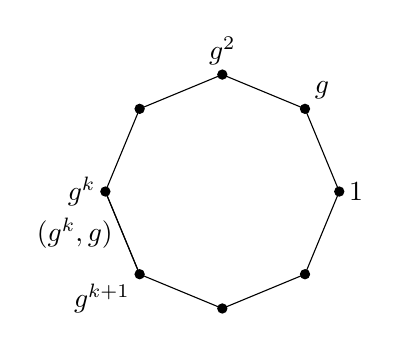
\begin{tikzpicture}[scale=1.1]
            \foreach \i in {0,...,7}{
                \coordinate (v\i) at ({360/8*\i}:1.35);
                \fill (v\i) circle (1.7pt);
            }

            \foreach \i/\j in {0/1,1/2,2/3,3/4,4/5,5/6,6/7,7/0}{
                \draw (v\i)--(v\j);
            }

            \node[right] at (v0) {\(1\)};
            \node[above right] at (v1) {\(g\)};
            \node[above] at (v2) {\(g^2\)};
            \node[left] at (v4) {\(g^k\)};
            \node[below left] at (v5) {\(g^{k+1}\)};

            \draw (v4)--node[left] {\((g^k,g)\)} (v5);
        \end{tikzpicture}
    \]

    Se invece \(G\) è infinito, otteniamo una retta bi-infinita:
    \[
        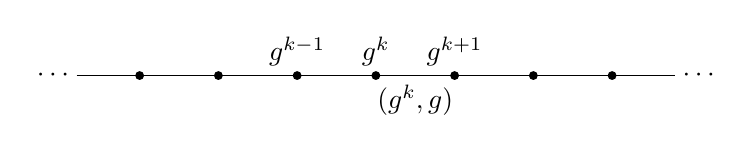
\begin{tikzpicture}[scale=1]
            \foreach \x in {-3,-2,-1,0,1,2,3}{
                \fill (\x,0) circle (1.6pt);
            }

            \draw (-3.8,0)--(3.8,0);
            \node at (-4.1,0) {\(\cdots\)};
            \node at (4.1,0) {\(\cdots\)};

            \node[above] at (-1,0) {\(g^{k-1}\)};
            \node[above] at (0,0) {\(g^k\)};
            \node[above] at (1,0) {\(g^{k+1}\)};

            \node[below] at (0.5,0) {\((g^k,g)\)};
        \end{tikzpicture}
    \]
\end{snippetexample}

\begin{snippetproposition}{Cappi e lati doppi nei grafi di Cayley}
    Sia \(\operatorname{Cay}(G,S)\) un grafo di Cayley.

    \begin{itemize}
        \item Ci sono cappi se e solo se \(1_G\in S\).
        \item Ci sono lati doppi se e solo se esiste \(s\in S\) tale che \(s^{-1}\in S\). Questo include il caso \(s=s^{-1}\), cioè \(s^2=1_G\).
    \end{itemize}
\end{snippetproposition}

\begin{snippetproof}{}
    Un lato \((g,s)\) è un cappio se e solo se i suoi estremi coincidono, cioè
    \[
        g=gs.
    \]
    Moltiplicando a sinistra per \(g^{-1}\), otteniamo \(s=1_G\). Quindi esistono cappi precisamente quando \(1_G\in S\).

    Consideriamo ora i lati doppi. Il lato \((g,s)\) congiunge \(g\) con \(gs\). Se anche \(s^{-1}\in S\), allora il lato \((gs,s^{-1})\) congiunge \(gs\) con
    \[
        (gs)s^{-1}=g.
    \]
    Quindi \((g,s)\) e \((gs,s^{-1})\) hanno gli stessi estremi.

    Viceversa, se due lati distinti hanno gli stessi estremi, allora uno deve corrispondere alla moltiplicazione per un elemento \(s\in S\) e l'altro alla moltiplicazione inversa, cioè per \(s^{-1}\). Dunque anche \(s^{-1}\in S\).
\end{snippetproof}

\begin{snippetexample}{Cappi e lati doppi}
    Se \(1_G\in S\), per ogni vertice \(g\) compare il cappio \((g,1_G)\).

    \[
        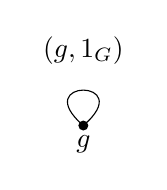
\begin{tikzpicture}[scale=1]
            \coordinate (g) at (0,0);
            \fill (g) circle (1.8pt);
            \node[below] at (g) {\(g\)};
            \draw (g) .. controls +(-0.7,0.6) and +(0.7,0.6) .. (g);
            \node[above] at (0,0.65) {\((g,1_G)\)};
        \end{tikzpicture}
    \]

    Se \(s,s^{-1}\in S\), compaiono due lati con gli stessi estremi:
    \[
        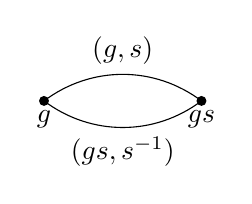
\begin{tikzpicture}[scale=1]
            \coordinate (g) at (0,0);
            \coordinate (h) at (2,0);

            \fill (g) circle (1.8pt);
            \fill (h) circle (1.8pt);

            \node[below] at (g) {\(g\)};
            \node[below] at (h) {\(gs\)};

            \draw (g) .. controls +(0.6,0.45) and +(-0.6,0.45) .. node[above] {\((g,s)\)} (h);
            \draw (g) .. controls +(0.6,-0.45) and +(-0.6,-0.45) .. node[below] {\((gs,s^{-1})\)} (h);
        \end{tikzpicture}
    \]
\end{snippetexample}

\begin{snippetproposition}{Componenti connesse del grafo di Cayley}
    Sia \(G\) un gruppo, sia \(S\subseteq G\) e poniamo
    \[
        H=\langle S\rangle.
    \]
    Allora la componente connessa di un vertice \(g\in G\) in \(\operatorname{Cay}(G,S)\) ha come insieme di vertici
    \[
        gH.
    \]
    In particolare, la componente connessa dell'identità \(1_G\) ha come vertici gli elementi di \(\langle S\rangle\).

    Di conseguenza,
    \[
        \operatorname{Cay}(G,S) \text{ è connesso}
        \quad\Longleftrightarrow\quad
        G=\langle S\rangle.
    \]
\end{snippetproposition}

\begin{snippetproof}{}
    Un lato del grafo permette di passare da un vertice \(x\) al vertice \(xs\), con \(s\in S\). Poiché il grafo è non orientato, attraversando lo stesso lato nel verso opposto si passa da \(xs\) a \(x\), cioè si moltiplica a destra per \(s^{-1}\).

    Quindi un cammino che parte da \(g\) e arriva in \(h\) corrisponde a una scrittura
    \[
        h=g s_1s_2\cdots s_r,
    \]
    dove ogni \(s_i\) appartiene a \(S\union S^{-1}\). Equivalentemente,
    \[
        g^{-1}h=s_1s_2\cdots s_r\in \langle S\rangle.
    \]
    Dunque \(h\in g\langle S\rangle\).

    Viceversa, se \(h\in g\langle S\rangle\), allora
    \[
        h=g s_1s_2\cdots s_r
    \]
    per certi \(s_i\in S\union S^{-1}\). Ogni moltiplicazione a destra per \(s_i\) corrisponde all'attraversamento di un lato del grafo, eventualmente nel verso opposto. Quindi esiste un cammino da \(g\) a \(h\).

    La componente connessa di \(g\) è perciò \(g\langle S\rangle\). Il grafo è connesso se e solo se tutti gli elementi di \(G\) appartengono alla componente dell'identità, cioè se e solo se
    \[
        G=\langle S\rangle.
    \]
\end{snippetproof}

\begin{snippetcorollary}{Componenti come laterali}
    Le componenti connesse di \(\operatorname{Cay}(G,S)\) sono i laterali sinistri di \(\langle S\rangle\):
    \[
        g\langle S\rangle,
        \qquad g\in G.
    \]
\end{snippetcorollary}

\begin{snippetproposition}{Circuiti nei grafi di Cayley}
    Il grafo di Cayley \(\operatorname{Cay}(G,S)\) contiene un circuito se e solo se esiste una parola non banale
    \[
        s_1s_2\cdots s_r=1_G,
        \qquad
        s_i\in S\union S^{-1},
    \]
    senza cancellazioni immediate, cioè tale che
    \[
        s_i s_{i+1}\neq 1_G
        \quad
        \text{per ogni } i.
    \]
    Per ottenere un circuito semplice bisogna inoltre richiedere che i prodotti parziali
    \[
        1_G,\ s_1,\ s_1s_2,\ \ldots,\ s_1s_2\cdots s_{r-1}
    \]
    siano tutti distinti.
\end{snippetproposition}

\begin{snippetproof}{}
    Supponiamo di avere una parola
    \[
        s_1s_2\cdots s_r=1_G,
        \qquad
        s_i\in S\union S^{-1}.
    \]
    Partendo da un vertice \(g\), consideriamo la successione di vertici
    \[
        g,\quad
        gs_1,\quad
        gs_1s_2,\quad
        \ldots,\quad
        gs_1s_2\cdots s_r.
    \]
    Poiché \(s_1s_2\cdots s_r=1_G\), l'ultimo vertice è di nuovo \(g\). Quindi otteniamo un cammino chiuso.

    La condizione \(s_i s_{i+1}\neq 1_G\) impedisce di percorrere un lato e subito dopo tornare indietro lungo lo stesso lato. Se inoltre i prodotti parziali sono tutti distinti, allora il cammino chiuso non ripete vertici intermedi e quindi è un circuito semplice.

    Viceversa, ogni circuito nel grafo di Cayley determina una sequenza di moltiplicazioni a destra per elementi di \(S\union S^{-1}\). Poiché il circuito torna al vertice di partenza, il prodotto corrispondente deve essere \(1_G\).
\end{snippetproof}

\end{document}